\subsection{Ballwurfmaschine}
Die Ballwurfmaschine funktioniert nach einem einfachen Konzept. Der Ball wird in eine Verengung geschoben und durch ein Drehrad nach vorne gedrückt. Dadurch wird er beschleunigt und zielgerichtet auf seine Flugbahn gelenkt.

\begin{figure}[h!]
\centering
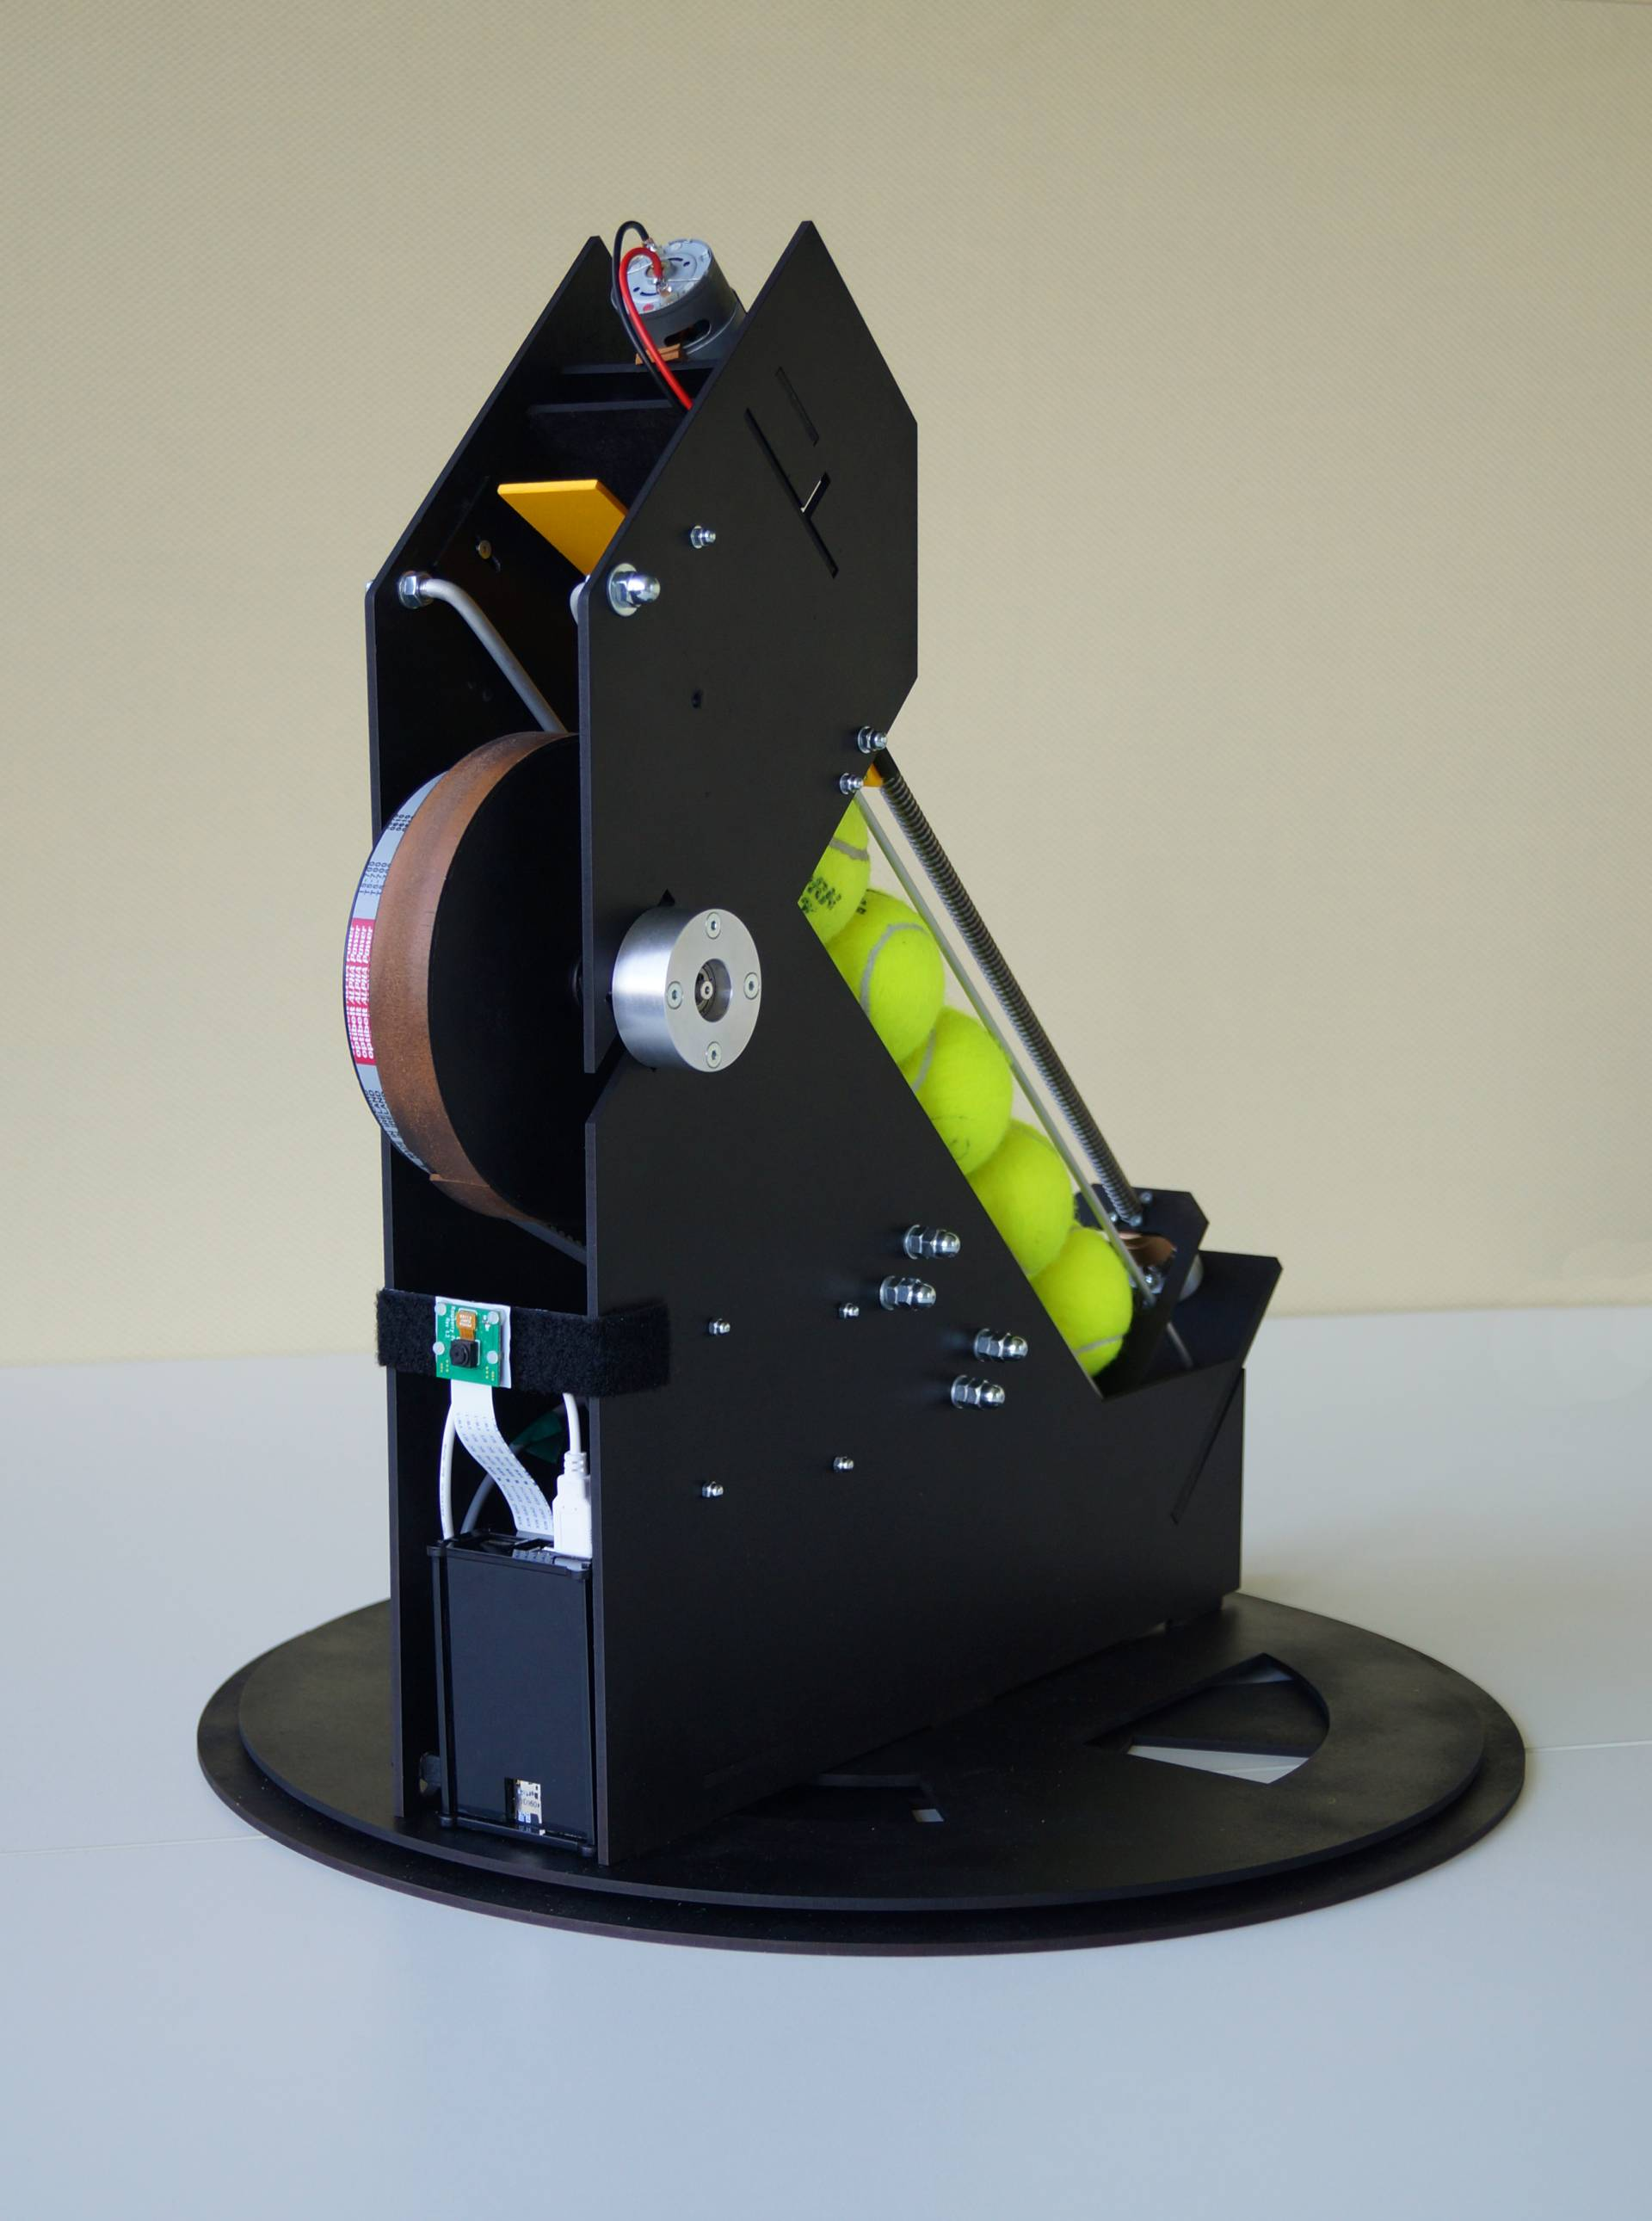
\includegraphics[width=0.7\linewidth]{../../fig/DSC08832xx}
\caption{Ballwurfmaschine Team 39}
\label{fig:ballwurfmaschine}
\end{figure}
